\documentclass[11pt,a4paper]{article}
\usepackage[utf8]{inputenc}
\usepackage[margin=1in]{geometry}
\usepackage{amsmath,amssymb}
\usepackage{hyperref}
\usepackage{booktabs}
\usepackage{longtable}
\usepackage{array}
\usepackage{tikz}
\usetikzlibrary{shapes.geometric, arrows.meta, positioning}

\title{\textbf{Technical Engine Specification: PLOS Backend}}
\author{\textbf{PLOS Core Architecture Team}}
\date{September 2026}

\begin{document}

\maketitle

\section{System Architecture Overview}

The PLOS backend is engineered following the Clean/Hexagonal Architecture pattern, enforcing a strict separation of concerns across software layers. The entire system is compiled into a single static binary targeting \textbf{Go 1.25.0}.

\begin{figure}[htbp]
\centering
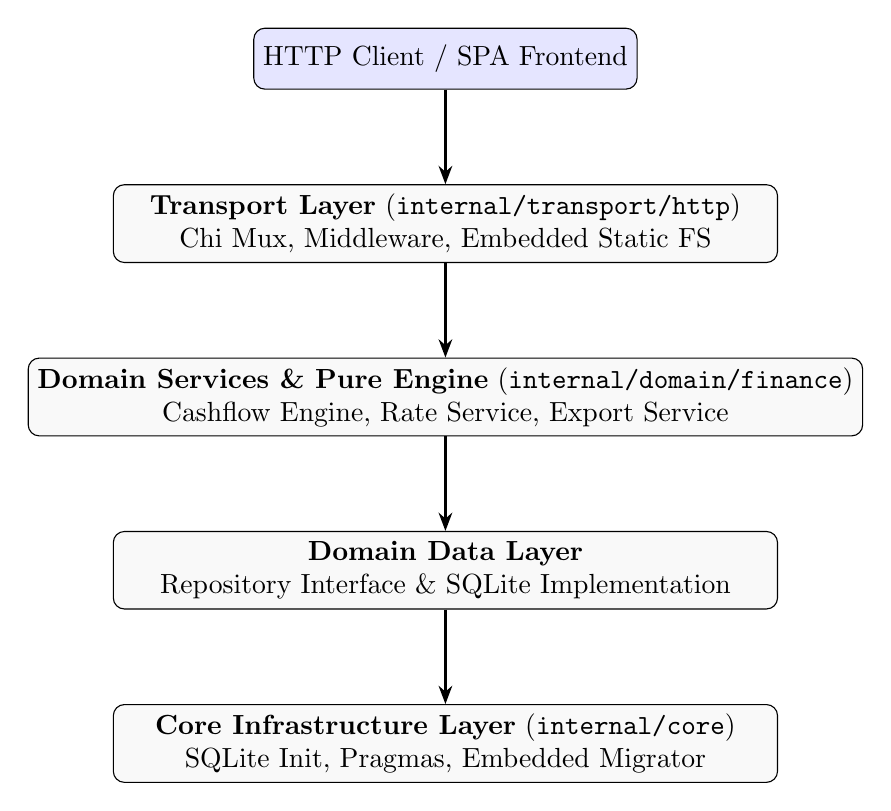
\begin{tikzpicture}[node distance=1.2cm, auto, >=Stealth]
    \tikzstyle{block} = [draw, fill=blue!10, rectangle, minimum height=2.2em, minimum width=12em, rounded corners, align=center]
    \tikzstyle{layer} = [draw, fill=gray!5, rectangle, minimum height=2.8em, minimum width=24em, rounded corners, align=center]

    \node [block] (client) {HTTP Client / SPA Frontend};
    \node [layer, below=of client] (transport) {\textbf{Transport Layer} (\texttt{internal/transport/http})\\Chi Mux, Middleware, Embedded Static FS};
    \node [layer, below=of transport] (domain) {\textbf{Domain Services \& Pure Engine} (\texttt{internal/domain/finance})\\Cashflow Engine, Rate Service, Export Service};
    \node [layer, below=of domain] (repo) {\textbf{Domain Data Layer}\\Repository Interface \& SQLite Implementation};
    \node [layer, below=of repo] (core) {\textbf{Core Infrastructure Layer} (\texttt{internal/core})\\SQLite Init, Pragmas, Embedded Migrator};

    \draw[->, thick] (client) -- (transport);
    \draw[->, thick] (transport) -- (domain);
    \draw[->, thick] (domain) -- (repo);
    \draw[->, thick] (repo) -- (core);
\end{tikzpicture}
\caption{PLOS Backend Hexagonal Architecture Execution Pipeline.}
\end{figure}

\subsection{Package Domain Responsibilities}

\noindent\begin{longtable}{@{\extracolsep{\fill}} l l p{7.5cm} @{}}
\toprule
\textbf{Package} & \textbf{Domain Area} & \textbf{Mechanical Purpose} \\ \midrule
\endhead
\bottomrule
\endfoot
\texttt{cmd/server} & Application Entrypoint & Initializes logger (\texttt{slog}), configuration, database pools, migrator, and HTTP server with graceful shutdown handling. \\
\texttt{internal/config} & Configuration & Loads runtime environment variables (\texttt{DB\_PATH}). \\
\texttt{internal/core} & Storage Infrastructure & Manages SQLite initialization, SQLite Pragmas, and transactional migration execution. \\
\texttt{internal/domain/finance} & Domain Models \& Logic & Defines domain entities, Repository contracts, SQLite repository, Rate service, and deterministic Cashflow Engine. \\
\texttt{internal/transport/http} & Transport / REST API & REST endpoints via \texttt{chi.Mux}, JSON serialization, request validation, and error handling. \\
\texttt{migrations} & Database Schemas & Versioned SQL migration files embedded directly into the binary using \texttt{embed.FS}. \\
\texttt{web} & Static Assets Integration & Holds embedded filesystem (\texttt{embed.FS}) of compiled frontend assets (\texttt{web/dist}). \\
\caption{Package responsibilities and layer bounds.}
\end{longtable}

\section{System Level \& Storage Subsystem Mechanics}

\subsection{SQLite Driver \& Database Connection Pool}

The system utilizes \texttt{modernc.org/sqlite}, a pure Go SQLite implementation, compiled statically. To leverage SQLite's Write-Ahead Logging (WAL) concurrency, the database connection pool is configured as:
\begin{equation}
\text{MaxOpenConns} = 10, \quad \text{MaxIdleConns} = 5, \quad \text{ConnMaxIdleTime} = 5\text{ minutes}
\end{equation}

\subsection{SQLite Hardware Sympathy Configuration (Pragmas)}

The database is initialized using optimal SQLite Pragmas tuned for SSD/NVMe storage mechanics:
\begin{itemize}
    \item \texttt{journal\_mode(WAL)}: Enables Write-Ahead Logging. Readers do not block writers, and writers do not block readers, achieving concurrent execution throughput.
    \item \texttt{synchronous(NORMAL)}: Eliminates unnecessary \texttt{fsync()} system calls on every transaction commit, syncing only during WAL checkpointing.
    \item \texttt{busy\_timeout(5000)}: Enforces an internal 5000ms retry backoff loop when lock contention occurs.
    \item \texttt{foreign\_keys(1)}: Enforces relational foreign key constraints on every mutation.
\end{itemize}

\section{Cashflow Engine Mechanics}

The \texttt{CashflowEngine} is a pure, deterministic domain engine processing monetary attributes using fixed-point integer cents (\texttt{int64}) to prevent IEEE-754 floating-point rounding inaccuracies.

\subsection{Mathematical Model of the Two-Phase Cascade Algorithm}

Foreign currency integer amounts $A_{\text{cents}}$ are normalized to base currency (EUR cents) using rounded division against $R_{\text{buy}}$:
\begin{equation}
A_{\text{EUR, cents}} = 
\begin{cases} 
A_{\text{cents}}, & \text{if Currency} = \text{EUR} \\ 
\left\lfloor \frac{A_{\text{cents}}}{R_{\text{buy}}} + 0.5 \right\rfloor, & \text{if Currency} = \text{UAH} 
\end{cases}
\end{equation}

The total available liquidity for the monthly period is calculated as:
\begin{equation}
C_{\text{avail, cents}} = \sum \text{Income}_{\text{EUR, cents}} - \sum \text{Expense}_{\text{EUR, cents}}
\end{equation}

\subsubsection{Phase A: Mandatory Minimum Payments}
For each active debt $d_i \in D$, mandatory minimum payments are applied in EUR cents:
\begin{equation}
P_{\text{min}, i} = \min\left(\text{MinPayment}_{\text{EUR, cents}}(d_i), \text{Remaining}_{\text{EUR, cents}}(d_i), C_{\text{avail, cents}}\right)
\end{equation}
\begin{equation}
\text{Remaining}_{\text{cents}}(d_i) \leftarrow \text{Remaining}_{\text{cents}}(d_i) - P_{\text{min, original}, i}
\end{equation}
\begin{equation}
C_{\text{avail, cents}} \leftarrow C_{\text{avail, cents}} - P_{\text{min}, i}
\end{equation}

\subsubsection{Phase B: Cascade Priority Surplus Distribution}
Iterating through active debts sorted in strict priority order ($P_1 \to P_n$), remaining available liquidity $C_{\text{avail, cents}}$ is cascaded:
\begin{equation}
P_{\text{extra}, k} = \min\left(C_{\text{avail, cents}}, \text{Remaining}_{\text{EUR, cents}}(d_k)\right)
\end{equation}
\begin{equation}
\text{Remaining}_{\text{cents}}(d_k) \leftarrow \text{Remaining}_{\text{cents}}(d_k) - P_{\text{extra, original}, k}
\end{equation}
\begin{equation}
C_{\text{avail, cents}} \leftarrow C_{\text{avail, cents}} - P_{\text{extra}, k}
\end{equation}

\subsubsection{Termination Condition}
Debt payoff state transitions strictly on exact integer thresholds:
\begin{equation}
\forall d_i \in D, \quad \text{if } \text{Remaining}_{\text{cents}}(d_i) \le 0 \implies \text{Remaining}_{\text{cents}}(d_i) = 0, \quad \text{Status}(d_i) = \text{PAID}
\end{equation}

\section{REST API Specification}

\noindent\begin{longtable}{@{\extracolsep{\fill}} l l l p{5.5cm} @{}}
\toprule
\textbf{HTTP Method} & \textbf{Endpoint Path} & \textbf{Status Code} & \textbf{Description / Purpose} \\ \midrule
\endhead
\bottomrule
\endfoot
\texttt{GET} & \texttt{/api/v1/currencies} & \texttt{200 OK} & Fetch supported ISO currencies. \\
\texttt{POST} & \texttt{/api/v1/currencies} & \texttt{201 Created} & Register a new ISO currency reference. \\
\texttt{GET} & \texttt{/api/v1/rates} & \texttt{200 OK} & Query latest exchange rates. \\
\texttt{POST} & \texttt{/api/v1/rates/sync} & \texttt{200 OK} & Trigger rate sync via Monobank Public API. \\
\texttt{POST} & \texttt{/api/v1/rates/manual} & \texttt{200 OK} & Set manual rate override. \\
\texttt{GET} & \texttt{/api/v1/accounts} & \texttt{200 OK} & Retrieve financial accounts list (\texttt{current\_balance\_cents}). \\
\texttt{POST} & \texttt{/api/v1/accounts} & \texttt{201 Created} & Create new financial account/category (\texttt{initial\_balance\_cents}). \\
\texttt{GET} & \texttt{/api/v1/debts} & \texttt{200 OK} & Get active debts ordered by priority ($P_1 \to P_n$). \\
\texttt{POST} & \texttt{/api/v1/debts} & \texttt{200 OK} & Upsert debt metadata attributes. \\
\texttt{POST} & \texttt{/api/v1/cashflow/simulate} & \texttt{200 OK} & Run one-step cascade payoff simulation (\texttt{amount\_cents}). \\
\texttt{GET} & \texttt{/api/v1/export/debts.csv} & \texttt{200 OK} & Export active debts as RFC 4180 CSV stream. \\
\caption{API Route Index and Endpoint Definitions.}
\end{longtable}

\end{document}
